\documentclass{mimosis}
\usepackage{vhistory}

\usepackage{metalogo}

\usepackage[final]{pdfpages}

\usepackage{etoolbox}
\usepackage[utf8]{inputenc}

\usepackage{tocloft}
\usepackage[titletoc]{appendix}

\usepackage{graphicx}
\graphicspath{{Pictures/}}

\usepackage[binary-units=true]{siunitx}
\DeclareSIUnit\px{px}

\usepackage{acro}
\acsetup{first-style=short}
% class `abbrev': abbreviations:
\DeclareAcronym{3d}{
    short = {3D} ,
    long  = {Drie dimensionaal} ,
    class = {abbrev}
}
\DeclareAcronym{2d}{
    short = {2D} ,
    long  = {Twee dimensionaal} ,
    class = {abbrev}
}
\DeclareAcronym{hdpe}{
    short = {HDPE} ,
    long  = {High-density polyethylene} ,
    foreign  = {Hogedichtheidpolyetheen} ,
    class = {abbrev}
}
\DeclareAcronym{am}{
    short = {AM} ,
    long  = {Additive manufacturing} ,
    foreign = {Additieve productie},
    class = {abbrev}
}
\DeclareAcronym{fdm}{
    short = {FDM} ,
    long  = {Gefuseerde depositiemodellering} ,
    foreign = {Fused deposition modeling},
    class = {abbrev}
}
\DeclareAcronym{fff}{
    short = {FDM} ,
    long  = {Fabricage van gesmolten filament} ,
    foreign = {Fused filament fabrication},
    class = {abbrev}
}
% class `nomencl': nomenclature
\DeclareAcronym{cpp}{
    short = {C++} ,
    long  = {programmeertaal gebaseerd op C} ,
    sort  = {cpp} ,
    class = {nomencl}
}
\DeclareAcronym{numofangels}{
    short = \ensuremath{N} ,
    long  = The number of angels per needle point ,
    sort  = N ,
    class = nomencl
}
\DeclareAcronym{areaofneedle}{
    short = \ensuremath{A} ,
    long  = The area of the needle point ,
    sort  = A ,
    class = nomencl
}
\DeclareAcronym{extruder}{
    short = {extruder} ,
    long  = {Het gedeelte van een FDM 3d printer waar het filament mee door het hotend en de nozel word geperst} ,
    sort  = {extruder} ,
    class = {nomencl}
}
\DeclareAcronym{hotend}{
    short = {hotend} ,
    long  = {Het gedeelte van een FDM 3d printer waar het filament smelt} ,
    sort  = {hotend} ,
    class = {nomencl}
}

\setlength{\cftbeforechapskip}{3pt}

\sisetup{%
  detect-all           = true,
  detect-family        = true,
  detect-mode          = true,
  detect-shape         = true,
  detect-weight        = true,
  detect-inline-weight = math,
}

\providecommand{\tightlist}{%
  \setlength{\itemsep}{0pt}\setlength{\parskip}{0pt}}

%%%%%%%%%%%%%%%%%%%%%%%%%%%%%%%%%%%%%%%%%%%%%%%%%%%%%%%%%%%%%%%%%%%%%%%%
% Hyperlinks & bookmarks
%%%%%%%%%%%%%%%%%%%%%%%%%%%%%%%%%%%%%%%%%%%%%%%%%%%%%%%%%%%%%%%%%%%%%%%%

\usepackage[%
  colorlinks = true,
  citecolor  = RoyalBlue,
  linkcolor  = RoyalBlue,
  urlcolor   = RoyalBlue,
  ]{hyperref}

\usepackage{bookmark}


%%%%%%%%%%%%%%%%%%%%%%%%%%%%%%%%%%%%%%%%%%%%%%%%%%%%%%%%%%%%%%%%%%%%%%%%
% Fonts
%%%%%%%%%%%%%%%%%%%%%%%%%%%%%%%%%%%%%%%%%%%%%%%%%%%%%%%%%%%%%%%%%%%%%%%%

\ifxetexorluatex
  \setmainfont{Minion Pro}
\else
  \usepackage[lf]{ebgaramond}
  \usepackage[oldstyle,scale=0.7]{sourcecodepro}
  \singlespacing
\fi

\renewcommand{\th}{\textsuperscript{\textup{th}}\xspace}

%pcb Printed circuit board
%mppt Maximum power point tracking
%spo2 Peripheral oxygen saturation

\newacronym{PCB}{PCB}{Printed circuit board}
\newacronym{MPPT}{MPPT}{Maximum power point tracking}
\newacronym{SPO2}{SPO2}{Peripheral oxygen saturation}
\newacronym{SMD}{SMD}{Surface-mounted Device}
\newacronym{USB}{USB}{Universal Serial Bus}

\makeindex
\makeglossaries

%%%%%%%%%%%%%%%%%%%%%%%%%%%%%%%%%%%%%%%%%%%%%%%%%%%%%%%%%%%%%%%%%%%%%%%%
% Incipit
%%%%%%%%%%%%%%%%%%%%%%%%%%%%%%%%%%%%%%%%%%%%%%%%%%%%%%%%%%%%%%%%%%%%%%%%

\title{Eindverslag \textbf{Stage 3devo}}
\subtitle{Verwarmde behuizing voor het 3D printen van HDPE en PP}
\author{Luca van Straaten (18073611)}

\begin{document}

\frontmatter
\begin{titlepage}
    \vspace*{5cm}
    \makeatletter
    \begin{center}
        \begin{Huge}
            \@title
        \end{Huge}\\[0.1cm]
        %
        \begin{Large}
            \@subtitle
        \end{Large}\\
        %
        \emph{door}\\
        \@author
        %
        \vfill
        Dit document is opgesteld voor de stage bij 3devo. Luca van
        Straaten is een student Elektrotechniek aan de Haagse Hogeschool te
        delft.\\
        \vspace{.5cm}
        Datum: \today\\
        Versie: V 0.1
    \end{center}
    \makeatother
\end{titlepage}

\newpage


\begin{versionhistory}
    \vhEntry{0.1}{08.09.2021}{Luca}{Document aangemaakt}
    %\vhEntry{0.2}{29.10.2021}{Luca}{Eerste opzet}
    %\vhEntry{0.2}{29.10.2021}{Luca}{Eerste opzet}
\end{versionhistory}

\chapter*{Voorwoord}
\addcontentsline{toc}{chapter}{Voorwoord}
%%%%%%%%%%%%%%%%%%%%%%%%%%%%%%%%%%%%%%%%%%%%%%%%%%%%%%%%%%%%%%%%%%%%%%%%

Dit ontwerpdocument is geschreven als documenatie van het eerste stagetraject
van luca van Straaten\\\\

Utrecht, September 2021\\Luca van Straaten


\chapter{Samenvatting}
\label{Samenvatting}
%%%%%%%%%%%%%%%%%%%%%%%%%%%%%%%%%%%%%%%%%%%%%%%%%%%%%%%%%%%%%%%%%%%%%%%%

\begin{center}
   \begin{minipage}{0.5\textwidth}
      \begin{small}
         Dit is het eindverslag voor de eerste stage van Luca van Straaten. De stage vond plaats van maandag 6 september tot en met vrijdag 12 november 2021 bij 3devo in Utrecht.
      \end{small}
   \end{minipage}
   \vspace{0.5cm}
\end{center}

%%%%%%%%%%%%%%%%%%%%%%%%%%%%%%%%%%%%%%%%%%%%%%%%%%%%%%%%%%%%%%%%%%%%%%%%
% \section{Section}
%%%%%%%%%%%%%%%%%%%%%%%%%%%%%%%%%%%%%%%%%%%%%%%%%%%%%%%%%%%%%%%%%%%%%%%%

%%%%%%%%%%%%%%%%%%%%%%%%%%%%%%%%%%%%%%%%%%%%%%%%%%%%%%%%%%%%%%%%%%%%%%%%
% \subsection{Subsection}
%%%%%%%%%%%%%%%%%%%%%%%%%%%%%%%%%%%%%%%%%%%%%%%%%%%%%%%%%%%%%%%%%%%%%%%%


%\begingroup
%    \let\clearpage\relax
%    \glsaddall
%    \printglossary[type=\acronymtype]
%    \addcontentsline{toc}{chapter}{Acroniemen}
%\endgroup
\newpage
\tableofcontents
\newpage
\listoffigures
\addcontentsline{toc}{chapter}{Lijst van figuren}

\printacronyms[include=abbrev,name=Lijst van afkortingen]
\printacronyms[include=nomencl,name=Lijst van begrippen]

\chapter{Inleiding}
\label{inleiding}
%%%%%%%%%%%%%%%%%%%%%%%%%%%%%%%%%%%%%%%%%%%%%%%%%%%%%%%%%%%%%%%%%%%%%%%%

\begin{center}
    \begin{minipage}{0.5\textwidth}
        \begin{small}
            Waar de reden tot creatie van dit verslag worden blootgelegd, en daarbij de opdracht en het probleem worden beschreven.
        \end{small}
    \end{minipage}
    \vspace{0.5cm}
\end{center}

\noindent De opdracht is om de aanstuur elecronica te maaken voor een 3D-printer die \ac{hdpe} kan printen.

%%%%%%%%%%%%%%%%%%%%%%%%%%%%%%%%%%%%%%%%%%%%%%%%%%%%%%%%%%%%%%%%%%%%%%%%
\section{Wat is 3D-printen}
%%%%%%%%%%%%%%%%%%%%%%%%%%%%%%%%%%%%%%%%%%%%%%%%%%%%%%%%%%%%%%%%%%%%%%%%

3D-printen is een additieve productie (\ac{am}) methode. Dat betekent dat een product word opgebouwd vanaf nul, in tegenstelling tot subtractieve productie is er weinig of geen verlies van materiaal.
Een andere vorm van additieve productie is bijvoorbeeld spuitgieten, maar hierbij zijn kostbare gietmallen nodig. 3D-printen vereist geen grote investering voor elk nieuw ontwerp, en is daarom uitermate geschikt om snel prototypen te maken. \cite{ATTARAN2017677}

%%%%%%%%%%%%%%%%%%%%%%%%%%%%%%%%%%%%%%%%%%%%%%%%%%%%%%%%%%%%%%%%%%%%%%%%
\subsection{\ac{fdm} 3D-printen}
%%%%%%%%%%%%%%%%%%%%%%%%%%%%%%%%%%%%%%%%%%%%%%%%%%%%%%%%%%%%%%%%%%%%%%%%

Er zijn verschillende vormen van 3D-printen, maar verreweg de meest populaire bij hobbyisten en kleinschalige bedrijven is FDM 3D-printen. FDM staat voor Fused deposition modeling, hierbij word steeds een laag materiaal op de vorige laag neergelegd (depositie) en daar op vast gesmolten (gefuseerd). Door herhaaldelijk laagjes op elkaar neer te leggen kan een \ac{3d} object woorden opgebouwd.

%%%%%%%%%%%%%%%%%%%%%%%%%%%%%%%%%%%%%%%%%%%%%%%%%%%%%%%%%%%%%%%%%%%%%%%%
\subsection{3D-printer software}
%%%%%%%%%%%%%%%%%%%%%%%%%%%%%%%%%%%%%%%%%%%%%%%%%%%%%%%%%%%%%%%%%%%%%%%%



%%%%%%%%%%%%%%%%%%%%%%%%%%%%%%%%%%%%%%%%%%%%%%%%%%%%%%%%%%%%%%%%%%%%%%%%
\subsection{3D-printer firmware}
%%%%%%%%%%%%%%%%%%%%%%%%%%%%%%%%%%%%%%%%%%%%%%%%%%%%%%%%%%%%%%%%%%%%%%%%

%%%%%%%%%%%%%%%%%%%%%%%%%%%%%%%%%%%%%%%%%%%%%%%%%%%%%%%%%%%%%%%%%%%%%%%%
\section{Wat is HDPE}
%%%%%%%%%%%%%%%%%%%%%%%%%%%%%%%%%%%%%%%%%%%%%%%%%%%%%%%%%%%%%%%%%%%%%%%%

%%%%%%%%%%%%%%%%%%%%%%%%%%%%%%%%%%%%%%%%%%%%%%%%%%%%%%%%%%%%%%%%%%%%%%%%
\section{Waarom HDPE}
%%%%%%%%%%%%%%%%%%%%%%%%%%%%%%%%%%%%%%%%%%%%%%%%%%%%%%%%%%%%%%%%%%%%%%%%

nylon, ceramics, wax, bronze, stainless steel, cobalt chrome and titanium.

%%%%%%%%%%%%%%%%%%%%%%%%%%%%%%%%%%%%%%%%%%%%%%%%%%%%%%%%%%%%%%%%%%%%%%%%
\section{Bestanden downloaden}
%%%%%%%%%%%%%%%%%%%%%%%%%%%%%%%%%%%%%%%%%%%%%%%%%%%%%%%%%%%%%%%%%%%%%%%%

Dit hele project is gewerkt in en is vast gelegd in git. Maar omdat de inhoud
van het project en verslag intellectueel eigendom is van 3devo, staat dat niet
openbaar op GitHub. Als je echter denkt recht te hebben op het inzien van de
bestanden (elektrische schema's, 3D bestanden, code, etc.) dan kunt u daar
beroep op doen door te mailen naar
\href{mailto:lucavanstraaten@icloud.com}{lucavanstraaten@icloud.com}


\mainmatter

\chapter{Analyse van het probleem}
\label{Analyse_van_het_probleem}
%%%%%%%%%%%%%%%%%%%%%%%%%%%%%%%%%%%%%%%%%%%%%%%%%%%%%%%%%%%%%%%%%%%%%%%%

\begin{center}
    \begin{minipage}{0.5\textwidth}
        \begin{small}
            Waar de noodzaak van dit project word blootgelegd.
        \end{small} 
    \end{minipage}
    \vspace{0.5cm}
\end{center}

Kortweg is het probleem dat er momenteel niet met \ac{hdpe} en \ac{pp} kan
woorden ge-3D-print. 3D-printen met \ac{hdpe} en \ac{pp} is wenselijk omdat deze
materialen overvloedig zijn is de huidige afvalstroom, en ze dus goedkoop
te verkrijgen zijn.\\

Een voorbeeld van hoogwaardig PP in de afvalstroom zijn verpakkingen van
medische goederen in ziekenhuizen.  3devo heeft \ac{pp} bakjes van een
oogheelkunde kliniek en wil dat recyclen tot 3D-printer filament. Zie Figuur
\ref{fig:pp_bakjes} voor de bakjes.

\begin{figure}[h]
    \centerline{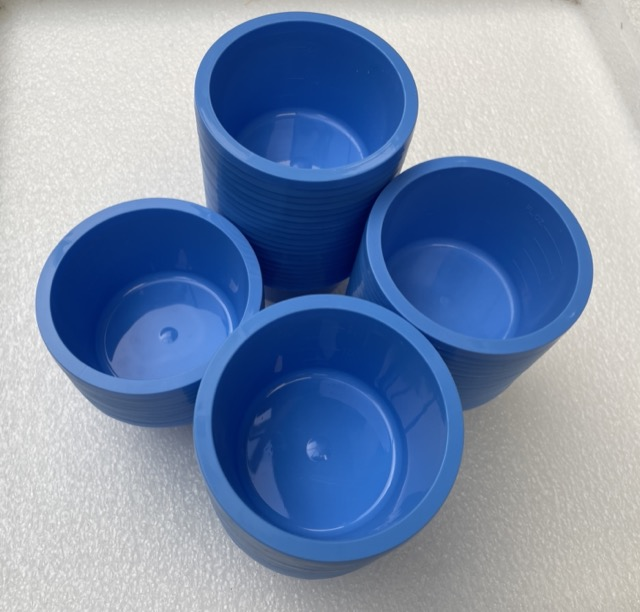
\includegraphics[width=0.4\textwidth]{pp_bakjes}}
    \caption{\ac{pp} bakjes van een oogheelkunde kliniek}
    \label{fig:pp_bakjes}
\end{figure}

%%%%%%%%%%%%%%%%%%%%%%%%%%%%%%%%%%%%%%%%%%%%%%%%%%%%%%%%%%%%%%%%%%%%%%%%
\section{Waarom is een speciale 3D-printer nodig}
%%%%%%%%%%%%%%%%%%%%%%%%%%%%%%%%%%%%%%%%%%%%%%%%%%%%%%%%%%%%%%%%%%%%%%%%

Er zijn twee redenen gegeven waarom een speciale printer nodig is voor het
printen met \ac{hdpe} en \ac{pp}.  Tests zijn uitgevoerd om vast te stellen of
deze complicaties werkelijk het printen van \ac{hdpe} en \ac{pp} onmogelijk
maken.

%%%%%%%%%%%%%%%%%%%%%%%%%%%%%%%%%%%%%%%%%%%%%%%%%%%%%%%%%%%%%%%%%%%%%%%%
\subsection{Printen op een conventionele 3D-printer}
%%%%%%%%%%%%%%%%%%%%%%%%%%%%%%%%%%%%%%%%%%%%%%%%%%%%%%%%%%%%%%%%%%%%%%%%

Er is een test uitgevoerd met het printen van \ac{hdpe} en \ac{pp}.  Deze test
zijn uitgevoerd op een conventionele \ac{fdm} 3D-printer, namelijk een Ender-3.
De slicer settings die gebruikt zijn waren vooral getweakt op temperatuur en
snelheid.

\begin{figure}[h]
    \centering
    \begin{minipage}{0.45\textwidth}
        \centerline{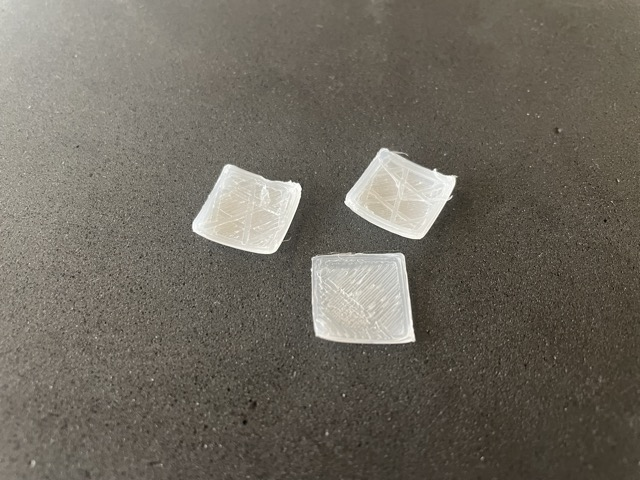
\includegraphics[width=0.9\textwidth]{hdpe_per_test}}
        \caption{Test print met \ac{hdpe} op een conventionele printer}
        \label{fig:hdpe_test}
    \end{minipage}\hfill
    \begin{minipage}{0.45\textwidth}
        \centerline{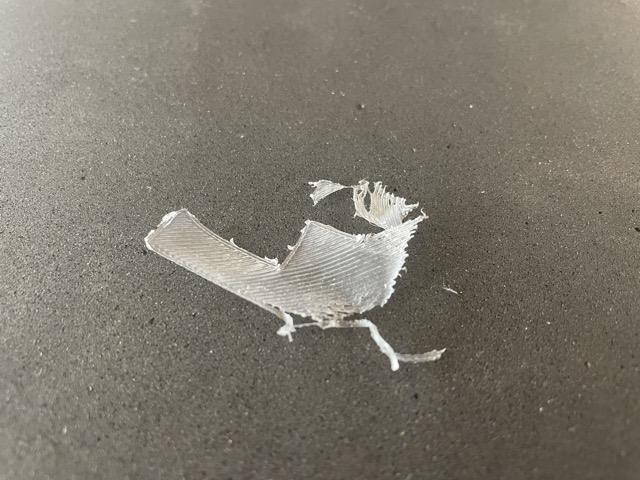
\includegraphics[width=0.9\textwidth]{pp_pre_test}}
        \caption{Test print met \ac{pp} op een conventionele printer}
        \label{fig:pp_test}
    \end{minipage}
\end{figure}

%%%%%%%%%%%%%%%%%%%%%%%%%%%%%%%%%%%%%%%%%%%%%%%%%%%%%%%%%%%%%%%%%%%%%%%%
\subsubsection{Laag hechting}
%%%%%%%%%%%%%%%%%%%%%%%%%%%%%%%%%%%%%%%%%%%%%%%%%%%%%%%%%%%%%%%%%%%%%%%%

De hypothese is dat bij het printen met \ac{pp} de laag hechting niet goed zal
zijn. Dat komt doordat \ac{pp} onder de kristallisatietemperatuur niet
''plakkerig'' is. De test met het printen van \ac{pp} heeft geconcludeerd dat
die hypothese waar is. Het materiaal blijft moeilijk plakken aan het bed, en als
dat goed ging, blijft het ook nauwelijks plakken aan zichzelf. Zie Figuur
\ref{fig:pp_test}. Een ander probleem met het printen van \ac{pp} is dat het
flexibele plastic niet goed door een bowden extruder gaat vanwege de extra
weerstand in dat systeem. Uitleg over wat een bowden tube extruder is staat in
hoofdstuk \ref{ss:Bowden_extruder}.

%%%%%%%%%%%%%%%%%%%%%%%%%%%%%%%%%%%%%%%%%%%%%%%%%%%%%%%%%%%%%%%%%%%%%%%%
\subsubsection{Krom trekken}
%%%%%%%%%%%%%%%%%%%%%%%%%%%%%%%%%%%%%%%%%%%%%%%%%%%%%%%%%%%%%%%%%%%%%%%%

De verwachting was dat het grote probleem met HDPE is dat het krom trekt tijdens
het printen. Tijdens het printen zal er een warmte gradiënt ontstaan, omdat de
laag die net is neergelegd al aan het afkoelen is voor dat de volgende de
volgende laag daar op word gelegd. Tijdens het testen op een conventionele
printer is vastgesteld dat dat inderdaad een probleem is, zie Figuur
\ref{fig:hdpe_test} voor een foto van de krom getrokken prints.

\chapter{Eisen van het project}
\label{Eisen_van_het_project}
%%%%%%%%%%%%%%%%%%%%%%%%%%%%%%%%%%%%%%%%%%%%%%%%%%%%%%%%%%%%%%%%%%%%%%%%

%%%%%%%%%%%%%%%%%%%%%%%%%%%%%%%%%%%%%%%%%%%%%%%%%%%%%%%%%%%%%%%%%%%%%%%%
\subsection{Randvoorwaarden}
% waar moet je je aan houden (en kan je vanuit het project niet veranderen)?
% Voorbeeld: wet- en regelgeving. De voorschriften van de accountant etc.
%%%%%%%%%%%%%%%%%%%%%%%%%%%%%%%%%%%%%%%%%%%%%%%%%%%%%%%%%%%%%%%%%%%%%%%%

Het frame van een ender-5, de motoren van de ender-5, de behuizing, de
warmte-elementen en de positie daar van waren allemaal al ontworpen voordat aan
het project was begonnen. Dus deze aspecten van het project konden in principe niet
veranderen.

%%%%%%%%%%%%%%%%%%%%%%%%%%%%%%%%%%%%%%%%%%%%%%%%%%%%%%%%%%%%%%%%%%%%%%%%
\subsection{Functionele wensen}
% wat moet het resultaat kunnen/doen?
% Voorbeeld: 10.000 liter per uur zuiveren; 2500 broden per dag bakken;
% 500 aankopen per uur kunnen verwerken etc.
%%%%%%%%%%%%%%%%%%%%%%%%%%%%%%%%%%%%%%%%%%%%%%%%%%%%%%%%%%%%%%%%%%%%%%%%

De verwarmde kamer van de printer moet maximaal \SI{160}{\celsius} kunnen
woorden en stabiel zijn bij elke ingestelde temperatuur

%%%%%%%%%%%%%%%%%%%%%%%%%%%%%%%%%%%%%%%%%%%%%%%%%%%%%%%%%%%%%%%%%%%%%%%%
\subsection{Gebruikerswensen}
% welke eisen stellen gebruikers aan het resultaat?
% Voorbeeld: gebruikers moeten maximaal 3 keer doorklikken op de website om bij de informatie te komen die ze zoeken
%%%%%%%%%%%%%%%%%%%%%%%%%%%%%%%%%%%%%%%%%%%%%%%%%%%%%%%%%%%%%%%%%%%%%%%%

De gebruikersinterface moet een eenvoudige en snelle manier zijn om de printer
te gebruiken, dat betekent in principe dat de printer op dezelfde manier te
bedienen moet zijn als de originele Ender-5

%%%%%%%%%%%%%%%%%%%%%%%%%%%%%%%%%%%%%%%%%%%%%%%%%%%%%%%%%%%%%%%%%%%%%%%%
\subsection{Ontwerpbeperkingen}
% eisen die te maken hebben met de bouw/constructie
% Voorbeeld: promotiefilmpje op Youtube mag maximaal 10 minuten lang zijn
%%%%%%%%%%%%%%%%%%%%%%%%%%%%%%%%%%%%%%%%%%%%%%%%%%%%%%%%%%%%%%%%%%%%%%%%

Het project moet woorden gedaan in 10 weken. Dus er kunnen geen onderdelen
woorden gebruikt met een lange levertijd.

De extruder en hotend kunnen niet op de conventionele manier woorden gekoeld
omdat dezen zich in de verwarmde kamer bevinden. Dus als blijkt dat dezen
gekoeld moeten woorden moet daar een andere oplossing voor woorden gevonden.
\chapter{Problemen}
\label{Problemen}
%%%%%%%%%%%%%%%%%%%%%%%%%%%%%%%%%%%%%%%%%%%%%%%%%%%%%%%%%%%%%%%%%%%%%%%%

Tijdens het project zijn eer paar problemen opgetreden. Dezen hadden allemaal
te maken met de extruder en dat daar geen plastic meer uit komt (vast liep).

%%%%%%%%%%%%%%%%%%%%%%%%%%%%%%%%%%%%%%%%%%%%%%%%%%%%%%%%%%%%%%%%%%%%%%%%
\section{Smeltend plastic in de extruder}
\label{s:smeltendplastic}
%%%%%%%%%%%%%%%%%%%%%%%%%%%%%%%%%%%%%%%%%%%%%%%%%%%%%%%%%%%%%%%%%%%%%%%%

Een probleem waar al vrij snel tegen aan werd geloopen is dat de extruder vast
liep door dat het plastic te vroeg smelten, met het gevolg er geen plastic meer uit de nozel kwam.
Dit gebeurde telkens rond de zelfde tijd na het starten van een print.

%%%%%%%%%%%%%%%%%%%%%%%%%%%%%%%%%%%%%%%%%%%%%%%%%%%%%%%%%%%%%%%%%%%%%%%%
\subsection{Oorzaak}
%%%%%%%%%%%%%%%%%%%%%%%%%%%%%%%%%%%%%%%%%%%%%%%%%%%%%%%%%%%%%%%%%%%%%%%%

Dit probleem was het resultaat van warme drive gears (extruder tandwielen).
Heat creep is een term voor het warmte gradiënt door de metalen onderdelen van
de extruder. De stappenmotor van de extruder en de heater cartridge van het
hotend produceren allebei warmte. Deze warmte geleid door de hele extruder
assemblage en komt dus ook bij de drive gears. Als daardoor het plastic ook
warm word smelt het in de extruder. En kan het dus niet meer door de nozel
woorden geperst.

%%%%%%%%%%%%%%%%%%%%%%%%%%%%%%%%%%%%%%%%%%%%%%%%%%%%%%%%%%%%%%%%%%%%%%%%
\section{Dubbelvouwend plastic in de extruder}
\label{s:Dubbelvouwend}
%%%%%%%%%%%%%%%%%%%%%%%%%%%%%%%%%%%%%%%%%%%%%%%%%%%%%%%%%%%%%%%%%%%%%%%%

Een probleem tijdens het testen met een PP print wat dat het plastic dubbel
vouwde in de ruimte tussen de extruder tandwielen en de glijder naar de
extruder. Dit is dus een ander probleem dan beschreven in hoofdstuk
\ref{s:smeltendplastic}, dit probleem treed eerder op en zelfs als de kamer
niet is verwarmd. Dit probleem treden ook op tijdens het testen van PP op een
normaale printer, echter om een andere reden.

%%%%%%%%%%%%%%%%%%%%%%%%%%%%%%%%%%%%%%%%%%%%%%%%%%%%%%%%%%%%%%%%%%%%%%%%
\subsection{Oorzaak}
%%%%%%%%%%%%%%%%%%%%%%%%%%%%%%%%%%%%%%%%%%%%%%%%%%%%%%%%%%%%%%%%%%%%%%%%

Dit komt doordat er genoeg ruimte is tussen de extruder tandwielen en het
extruder frame dat er filament tussen door past. En omdat PP veel flexibeler is
dan HDPE, gaat het makkelijk daar tussen zitten.

Dit probleem had een adere oorzaak bij het testen op een standaard ender-3. De
oorzaak was echter dat de extruder veel meer kracht zou moeten zetten omdat de
ender-3 een bowden extruder printer is. Uitleg over wat een bowden tube
extruder is staat in hoofdstuk \ref{ss:Bowden_extruder}.


%%%%%%%%%%%%%%%%%%%%%%%%%%%%%%%%%%%%%%%%%%%%%%%%%%%%%%%%%%%%%%%%%%%%%%%%
\section{kamer temperatuur overshoot}
%%%%%%%%%%%%%%%%%%%%%%%%%%%%%%%%%%%%%%%%%%%%%%%%%%%%%%%%%%%%%%%%%%%%%%%%

De temperatuur van de verwarmde kamer schiet door het setpoint heen voordat het
stabiliseert of oscilleert rond de ingestelde waarden

%%%%%%%%%%%%%%%%%%%%%%%%%%%%%%%%%%%%%%%%%%%%%%%%%%%%%%%%%%%%%%%%%%%%%%%%
\subsection{Oorzaak}
%%%%%%%%%%%%%%%%%%%%%%%%%%%%%%%%%%%%%%%%%%%%%%%%%%%%%%%%%%%%%%%%%%%%%%%%

De massa van de thermistor is zo hoog dat het lang duurt om in evenwicht te
komen met de luchttemperatuur. Daarom loopt de gemeenten temperatuur dus
aanzienlijk achter op de werkelijke temperatuur. De werkelijke temperatuur is
geverifieerd door een thermokoppel naast de thermistor te hangen.
\chapter{Mogelijke oplossingen}
\label{Mogelijke_oplossingen}
%%%%%%%%%%%%%%%%%%%%%%%%%%%%%%%%%%%%%%%%%%%%%%%%%%%%%%%%%%%%%%%%%%%%%%%%

%%%%%%%%%%%%%%%%%%%%%%%%%%%%%%%%%%%%%%%%%%%%%%%%%%%%%%%%%%%%%%%%%%%%%%%%
\section{Extruder problemen}
%%%%%%%%%%%%%%%%%%%%%%%%%%%%%%%%%%%%%%%%%%%%%%%%%%%%%%%%%%%%%%%%%%%%%%%%

Het probleem van een vastlopende extruder kwam voor met een direct drive
extruder. Een oplossing die overwogen was, was het overstappen naar een andere
extruder architectuur.

%%%%%%%%%%%%%%%%%%%%%%%%%%%%%%%%%%%%%%%%%%%%%%%%%%%%%%%%%%%%%%%%%%%%%%%%
\subsection{Verschillende soorten extruders}
%%%%%%%%%%%%%%%%%%%%%%%%%%%%%%%%%%%%%%%%%%%%%%%%%%%%%%%%%%%%%%%%%%%%%%%%

\begin{figure}[h]
    \centerline{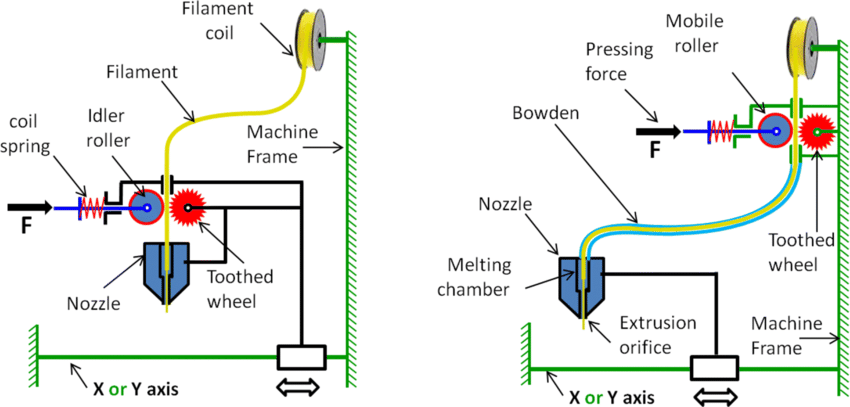
\includegraphics[width=0.85\textwidth]{Basic-diagram-of-FDM-3D-printer-extruder-a-Direct-extruder-b-Bowden-extruder}}
    \caption{Diagram van de twee soorten extruders die veel woorden gebruikt \cite{soorten_extruders}.}
    \label{fig:soorten_extruders}
\end{figure}

%%%%%%%%%%%%%%%%%%%%%%%%%%%%%%%%%%%%%%%%%%%%%%%%%%%%%%%%%%%%%%%%%%%%%%%%
\subsubsection{Bowden extruder}
\label{ss:Bowden_extruder}
%%%%%%%%%%%%%%%%%%%%%%%%%%%%%%%%%%%%%%%%%%%%%%%%%%%%%%%%%%%%%%%%%%%%%%%%

De rechter helft van Figuur \ref{fig:soorten_extruders} \cite{soorten_extruders}
is een diagram van een Bowden extruder. Hierbij is te zien dat \ac{extruder} los
is van de \ac{hotend}.

% uitleg

%%%%%%%%%%%%%%%%%%%%%%%%%%%%%%%%%%%%%%%%%%%%%%%%%%%%%%%%%%%%%%%%%%%%%%%%
\subsubsection{Direct drive extruder}
\label{ss:direct_drive_extruder}
%%%%%%%%%%%%%%%%%%%%%%%%%%%%%%%%%%%%%%%%%%%%%%%%%%%%%%%%%%%%%%%%%%%%%%%%

De linker helft van Figuur \ref{fig:soorten_extruders} \cite{soorten_extruders}
is een diagram van een direct drive extruder.

% uitleg

%%%%%%%%%%%%%%%%%%%%%%%%%%%%%%%%%%%%%%%%%%%%%%%%%%%%%%%%%%%%%%%%%%%%%%%%
\subsection{Zou een Bowden extruder de problemen oplossen}
%%%%%%%%%%%%%%%%%%%%%%%%%%%%%%%%%%%%%%%%%%%%%%%%%%%%%%%%%%%%%%%%%%%%%%%%

Met een bowden extruder zou het probleem van smeltend plastic in de extruder
(Hoofdstuk \ref{s:smeltendplastic}) opgelost kunnen woorden. Echter was
opgemerkt dat PP niet geprint kan woorden met een bowden printer (Hoofdstuk
\ref{s:Dubbelvouwend}).

%%%%%%%%%%%%%%%%%%%%%%%%%%%%%%%%%%%%%%%%%%%%%%%%%%%%%%%%%%%%%%%%%%%%%%%%
\subsection{Zou een water gekoelde extruder de problemen oplossen}
%%%%%%%%%%%%%%%%%%%%%%%%%%%%%%%%%%%%%%%%%%%%%%%%%%%%%%%%%%%%%%%%%%%%%%%%

Een water gekoelde extruder/hotend zou allebei de problemen kunnen oplossen met
als enige nadeel extra complexheid in de vorm van aanstuur elektronica en
software voor de waterkoeling en de waterkoeling zelf (buizen, pomp, radiator).

Een goede optie zou de "Titan Aqua" \cite{titanaqua} zijn.

% bronvermedling naar pagina over watergekoelde hotend/extruder

%%%%%%%%%%%%%%%%%%%%%%%%%%%%%%%%%%%%%%%%%%%%%%%%%%%%%%%%%%%%%%%%%%%%%%%%
\section{Temperatuur overshoot}
%%%%%%%%%%%%%%%%%%%%%%%%%%%%%%%%%%%%%%%%%%%%%%%%%%%%%%%%%%%%%%%%%%%%%%%%

Een \ac{PID} lus voor de kamertemperatuur kan woorden geïmplementeerd in de
firmware van de printer, het vermogen van de warmte-elementen kan worden
teruggedraaid om ervoor te zorgen dat de temperatuur minder snel stijgt en er
dus een minder groot verschil is tussen de gemeenten en de werkelijke
temperatuur.

\chapter{De gekozen oplossing}
\label{De_gekozen_oplossing}
%%%%%%%%%%%%%%%%%%%%%%%%%%%%%%%%%%%%%%%%%%%%%%%%%%%%%%%%%%%%%%%%%%%%%%%%

%%%%%%%%%%%%%%%%%%%%%%%%%%%%%%%%%%%%%%%%%%%%%%%%%%%%%%%%%%%%%%%%%%%%%%%%
% \section{Section}
%%%%%%%%%%%%%%%%%%%%%%%%%%%%%%%%%%%%%%%%%%%%%%%%%%%%%%%%%%%%%%%%%%%%%%%%

%%%%%%%%%%%%%%%%%%%%%%%%%%%%%%%%%%%%%%%%%%%%%%%%%%%%%%%%%%%%%%%%%%%%%%%%
% \subsection{Subsection}
%%%%%%%%%%%%%%%%%%%%%%%%%%%%%%%%%%%%%%%%%%%%%%%%%%%%%%%%%%%%%%%%%%%%%%%%


\chapter{Ontwerp van de oplossing en de benodigde onderdelen}
\label{Ontwerp_van_de_oplossing_en_de_benodigde_onderdelen}
%%%%%%%%%%%%%%%%%%%%%%%%%%%%%%%%%%%%%%%%%%%%%%%%%%%%%%%%%%%%%%%%%%%%%%%%

%%%%%%%%%%%%%%%%%%%%%%%%%%%%%%%%%%%%%%%%%%%%%%%%%%%%%%%%%%%%%%%%%%%%%%%%
\section{Hardware}
%%%%%%%%%%%%%%%%%%%%%%%%%%%%%%%%%%%%%%%%%%%%%%%%%%%%%%%%%%%%%%%%%%%%%%%%

het mechanich ontwerp van de printer was grotendeels al gedaan, echter zijn er een aantal aanpassingen gedaan, die staan hier beschreven

%%%%%%%%%%%%%%%%%%%%%%%%%%%%%%%%%%%%%%%%%%%%%%%%%%%%%%%%%%%%%%%%%%%%%%%%
\subsection{Ge-3D-printe oplossingen}
%%%%%%%%%%%%%%%%%%%%%%%%%%%%%%%%%%%%%%%%%%%%%%%%%%%%%%%%%%%%%%%%%%%%%%%%

Een aantal problemen zijn opgelost door kleine onderdelen te 3d printen. hier zijn
daar een paar voorbeelden van.

%%%%%%%%%%%%%%%%%%%%%%%%%%%%%%%%%%%%%%%%%%%%%%%%%%%%%%%%%%%%%%%%%%%%%%%%
\subsubsection{Voetjes van de printer}
%%%%%%%%%%%%%%%%%%%%%%%%%%%%%%%%%%%%%%%%%%%%%%%%%%%%%%%%%%%%%%%%%%%%%%%%

De voetjes van de printer waren te kort, dus daar zijn langere voor
ontworpen en ge-3D-print. Zie Figuur ~\ref{fig:voetjes} voor een render van
het \ac{3d} ontwerp.

\begin{figure}[h]
    \centerline{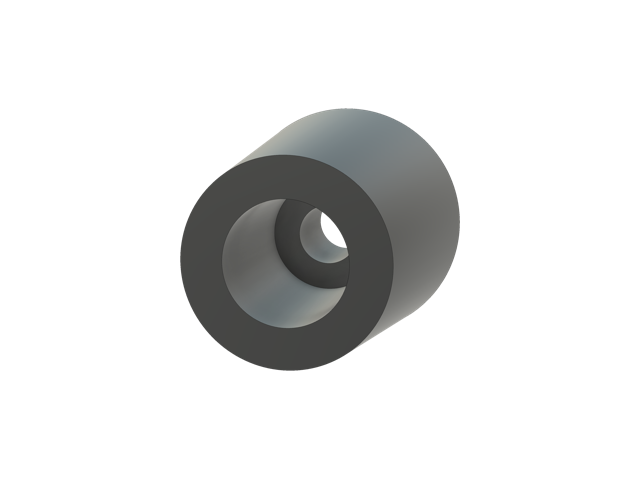
\includegraphics[width=0.45\textwidth]{voetjes}}
    \caption{Render van het \ac{3d} ontwerp van de voetjes van de printer}
    \label{fig:voetjes}
\end{figure}

%%%%%%%%%%%%%%%%%%%%%%%%%%%%%%%%%%%%%%%%%%%%%%%%%%%%%%%%%%%%%%%%%%%%%%%%
\subsubsection{Afstandhouder}
%%%%%%%%%%%%%%%%%%%%%%%%%%%%%%%%%%%%%%%%%%%%%%%%%%%%%%%%%%%%%%%%%%%%%%%%

De originele printer is omgebouwd met roestvrijstalen panelen aan alle kanten.
Om ervoor te zorgen dat er goede thermische isolatie is van de print kamer, is
het een dubbelwandig ontwerp met glaswol er tussen. De dubbele wanden worden op
afstand gehouden met ge-3D-printe afstandhouders. Zie Figuur
~\ref{fig:afstandhouder} voor een render van het \ac{3d} ontwerp van deze
afstandhouders.

%%%%%%%%%%%%%%%%%%%%%%%%%%%%%%%%%%%%%%%%%%%%%%%%%%%%%%%%%%%%%%%%%%%%%%%%
\subsubsection{Haakje}
%%%%%%%%%%%%%%%%%%%%%%%%%%%%%%%%%%%%%%%%%%%%%%%%%%%%%%%%%%%%%%%%%%%%%%%%

Om de deur dicht te houden is er een haakje geprint. Zie Figuur
~\ref{fig:haakje} voor een render van het \ac{3d} ontwerp van het haakje.

\begin{figure}[h]
    \centering
    \begin{minipage}{0.45\textwidth}
        \centerline{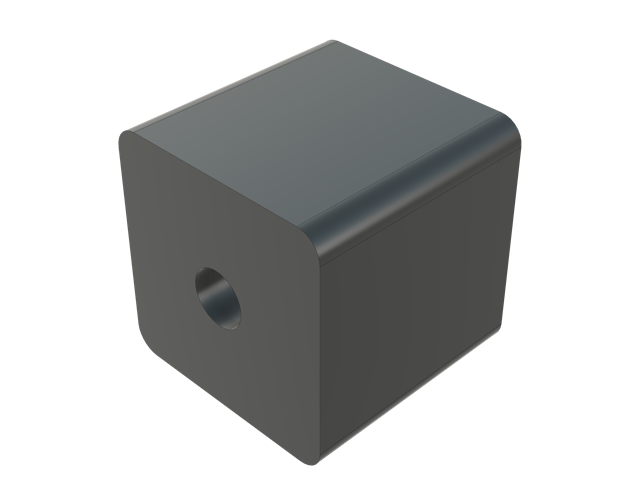
\includegraphics[width=0.9\textwidth]{afstandhouder}}
        \caption{Render van het \ac{3d} ontwerp van de afstandhouder van de printer}
        \label{fig:afstandhouder}
    \end{minipage}\hfill
    \begin{minipage}{0.45\textwidth}
        \centerline{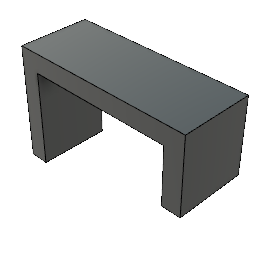
\includegraphics[width=0.9\textwidth]{haakje}}
        \caption{Render van het \ac{3d} ontwerp van het haakje van de printer}
        \label{fig:haakje}
    \end{minipage}
\end{figure}

%%%%%%%%%%%%%%%%%%%%%%%%%%%%%%%%%%%%%%%%%%%%%%%%%%%%%%%%%%%%%%%%%%%%%%%%
\section{Electronica}
%%%%%%%%%%%%%%%%%%%%%%%%%%%%%%%%%%%%%%%%%%%%%%%%%%%%%%%%%%%%%%%%%%%%%%%%

De te gebruiken electronica was grootendeels al vastgesteld voor het project begon.

%%%%%%%%%%%%%%%%%%%%%%%%%%%%%%%%%%%%%%%%%%%%%%%%%%%%%%%%%%%%%%%%%%%%%%%%
\section{Software}
%%%%%%%%%%%%%%%%%%%%%%%%%%%%%%%%%%%%%%%%%%%%%%%%%%%%%%%%%%%%%%%%%%%%%%%%

%%%%%%%%%%%%%%%%%%%%%%%%%%%%%%%%%%%%%%%%%%%%%%%%%%%%%%%%%%%%%%%%%%%%%%%%
\section{Firmware}
%%%%%%%%%%%%%%%%%%%%%%%%%%%%%%%%%%%%%%%%%%%%%%%%%%%%%%%%%%%%%%%%%%%%%%%%

%%%%%%%%%%%%%%%%%%%%%%%%%%%%%%%%%%%%%%%%%%%%%%%%%%%%%%%%%%%%%%%%%%%%%%%%
% \subsection{Subsection}
%%%%%%%%%%%%%%%%%%%%%%%%%%%%%%%%%%%%%%%%%%%%%%%%%%%%%%%%%%%%%%%%%%%%%%%%


\chapter{Assemblage van de oplossing}
\label{Assemblage_van_de_oplossing}
%%%%%%%%%%%%%%%%%%%%%%%%%%%%%%%%%%%%%%%%%%%%%%%%%%%%%%%%%%%%%%%%%%%%%%%%

%%%%%%%%%%%%%%%%%%%%%%%%%%%%%%%%%%%%%%%%%%%%%%%%%%%%%%%%%%%%%%%%%%%%%%%%
% \section{Section}
%%%%%%%%%%%%%%%%%%%%%%%%%%%%%%%%%%%%%%%%%%%%%%%%%%%%%%%%%%%%%%%%%%%%%%%%

%%%%%%%%%%%%%%%%%%%%%%%%%%%%%%%%%%%%%%%%%%%%%%%%%%%%%%%%%%%%%%%%%%%%%%%%
% \subsection{Subsection}
%%%%%%%%%%%%%%%%%%%%%%%%%%%%%%%%%%%%%%%%%%%%%%%%%%%%%%%%%%%%%%%%%%%%%%%%


\chapter{Ondervonden problemen}
\label{Ondervonden_problemen}
%%%%%%%%%%%%%%%%%%%%%%%%%%%%%%%%%%%%%%%%%%%%%%%%%%%%%%%%%%%%%%%%%%%%%%%%

% drive gears overtemp
% heated chaimber to much overshoot (oplosing 1, verminder vermogen van heraters. oplosing 2 implementeer pid lus)
%
%

%%%%%%%%%%%%%%%%%%%%%%%%%%%%%%%%%%%%%%%%%%%%%%%%%%%%%%%%%%%%%%%%%%%%%%%%
%\section{Hardware}
%%%%%%%%%%%%%%%%%%%%%%%%%%%%%%%%%%%%%%%%%%%%%%%%%%%%%%%%%%%%%%%%%%%%%%%%

%%%%%%%%%%%%%%%%%%%%%%%%%%%%%%%%%%%%%%%%%%%%%%%%%%%%%%%%%%%%%%%%%%%%%%%%
%\section{Electronica}
%%%%%%%%%%%%%%%%%%%%%%%%%%%%%%%%%%%%%%%%%%%%%%%%%%%%%%%%%%%%%%%%%%%%%%%%

%%%%%%%%%%%%%%%%%%%%%%%%%%%%%%%%%%%%%%%%%%%%%%%%%%%%%%%%%%%%%%%%%%%%%%%%
%\section{Software}
%%%%%%%%%%%%%%%%%%%%%%%%%%%%%%%%%%%%%%%%%%%%%%%%%%%%%%%%%%%%%%%%%%%%%%%%


\chapter{Eindresultaat}
\label{Eindresultaat}
%%%%%%%%%%%%%%%%%%%%%%%%%%%%%%%%%%%%%%%%%%%%%%%%%%%%%%%%%%%%%%%%%%%%%%%%

%%%%%%%%%%%%%%%%%%%%%%%%%%%%%%%%%%%%%%%%%%%%%%%%%%%%%%%%%%%%%%%%%%%%%%%%
%\section{Hardware}
%%%%%%%%%%%%%%%%%%%%%%%%%%%%%%%%%%%%%%%%%%%%%%%%%%%%%%%%%%%%%%%%%%%%%%%%

%%%%%%%%%%%%%%%%%%%%%%%%%%%%%%%%%%%%%%%%%%%%%%%%%%%%%%%%%%%%%%%%%%%%%%%%
%\section{Electronica}
%%%%%%%%%%%%%%%%%%%%%%%%%%%%%%%%%%%%%%%%%%%%%%%%%%%%%%%%%%%%%%%%%%%%%%%%

%%%%%%%%%%%%%%%%%%%%%%%%%%%%%%%%%%%%%%%%%%%%%%%%%%%%%%%%%%%%%%%%%%%%%%%%
%\section{Software}
%%%%%%%%%%%%%%%%%%%%%%%%%%%%%%%%%%%%%%%%%%%%%%%%%%%%%%%%%%%%%%%%%%%%%%%%

%%%%%%%%%%%%%%%%%%%%%%%%%%%%%%%%%%%%%%%%%%%%%%%%%%%%%%%%%%%%%%%%%%%%%%%%
% \subsection{Subsection}
%%%%%%%%%%%%%%%%%%%%%%%%%%%%%%%%%%%%%%%%%%%%%%%%%%%%%%%%%%%%%%%%%%%%%%%%


\chapter{Toetsing eindresultaat aan de hand van de eisen}
\label{Toetsing_eindresultaat_aan_de_hand_van_de_eisen}
%%%%%%%%%%%%%%%%%%%%%%%%%%%%%%%%%%%%%%%%%%%%%%%%%%%%%%%%%%%%%%%%%%%%%%%%

%%%%%%%%%%%%%%%%%%%%%%%%%%%%%%%%%%%%%%%%%%%%%%%%%%%%%%%%%%%%%%%%%%%%%%%%
\section{Veiligheid}
%%%%%%%%%%%%%%%%%%%%%%%%%%%%%%%%%%%%%%%%%%%%%%%%%%%%%%%%%%%%%%%%%%%%%%%%

Er is rekening gehouden met de elektrische veiligheid, in figuur
~\ref{fig:din3} is bijvoorbeeld te zien hoe een extra kapje is toegevoegd over
de blote contacten van de C-14 stekker.

%%%%%%%%%%%%%%%%%%%%%%%%%%%%%%%%%%%%%%%%%%%%%%%%%%%%%%%%%%%%%%%%%%%%%%%%
\section{Eenvoudigheid}
%%%%%%%%%%%%%%%%%%%%%%%%%%%%%%%%%%%%%%%%%%%%%%%%%%%%%%%%%%%%%%%%%%%%%%%%

De printer is makkelijk te gebruiken aan de hand van de handleiding, zie bijlage \ref{overdracht}.

%%%%%%%%%%%%%%%%%%%%%%%%%%%%%%%%%%%%%%%%%%%%%%%%%%%%%%%%%%%%%%%%%%%%%%%%
\section{Overig}
%%%%%%%%%%%%%%%%%%%%%%%%%%%%%%%%%%%%%%%%%%%%%%%%%%%%%%%%%%%%%%%%%%%%%%%%

De printer voldoet ook aan de andere eisen.

%%%%%%%%%%%%%%%%%%%%%%%%%%%%%%%%%%%%%%%%%%%%%%%%%%%%%%%%%%%%%%%%%%%%%%%%
% \subsection{Subsection}
%%%%%%%%%%%%%%%%%%%%%%%%%%%%%%%%%%%%%%%%%%%%%%%%%%%%%%%%%%%%%%%%%%%%%%%%

\chapter{Conclusie en aanbevelingen}
\label{Conclusie_en_aanbevelingen}
%%%%%%%%%%%%%%%%%%%%%%%%%%%%%%%%%%%%%%%%%%%%%%%%%%%%%%%%%%%%%%%%%%%%%%%%

%%%%%%%%%%%%%%%%%%%%%%%%%%%%%%%%%%%%%%%%%%%%%%%%%%%%%%%%%%%%%%%%%%%%%%%%
\section{Section}
%%%%%%%%%%%%%%%%%%%%%%%%%%%%%%%%%%%%%%%%%%%%%%%%%%%%%%%%%%%%%%%%%%%%%%%%

%%%%%%%%%%%%%%%%%%%%%%%%%%%%%%%%%%%%%%%%%%%%%%%%%%%%%%%%%%%%%%%%%%%%%%%%
\subsection{Subsection}
%%%%%%%%%%%%%%%%%%%%%%%%%%%%%%%%%%%%%%%%%%%%%%%%%%%%%%%%%%%%%%%%%%%%%%%%


\chapter{Evaluatie}
\label{Evaluatie}
%%%%%%%%%%%%%%%%%%%%%%%%%%%%%%%%%%%%%%%%%%%%%%%%%%%%%%%%%%%%%%%%%%%%%%%%

%%%%%%%%%%%%%%%%%%%%%%%%%%%%%%%%%%%%%%%%%%%%%%%%%%%%%%%%%%%%%%%%%%%%%%%%
\section{Section}
%%%%%%%%%%%%%%%%%%%%%%%%%%%%%%%%%%%%%%%%%%%%%%%%%%%%%%%%%%%%%%%%%%%%%%%%

%%%%%%%%%%%%%%%%%%%%%%%%%%%%%%%%%%%%%%%%%%%%%%%%%%%%%%%%%%%%%%%%%%%%%%%%
\subsection{Subsection}
%%%%%%%%%%%%%%%%%%%%%%%%%%%%%%%%%%%%%%%%%%%%%%%%%%%%%%%%%%%%%%%%%%%%%%%%



% This ensures that the subsequent sections are being included as root
% items in the bookmark structure of your PDF reader.
\bookmarksetup{startatroot}

\bibliographystyle{IEEEtran}
\bibliography{bronnen}

\begin{appendices}
\appendixpage
\noappendicestocpagenum
\addappheadtotoc
% \chapter{Elektrisch schema}
% \includepdf[pages=-,fitpaper,rotateoversize]{Appendices/schema_v2.pdf}
% \chapter{Ontwerp PCB}
% \includepdf[pages=-,fitpaper,rotateoversize]{Appendices/pcb_v2.pdf}
\end{appendices}

\backmatter
\end{document}
